%%%%%%%%%%%%%%%%%%%%%%%%%%%%%%%%%%%%%%%%%%%%%%%%%%%%%%%%%%%%%%%%%%%%%%%%
%    INSTITUTE OF PHYSICS PUBLISHING                                   %
%                                                                      %
%   `Preparing an article for publication in an Institute of Physics   %
%    Publishing journal using LaTeX'                                   %
%                                                                      %
%    LaTeX source code `ioplau2e.tex' used to generate `author         %
%    guidelines', the documentation explaining and demonstrating use   %
%    of the Institute of Physics Publishing LaTeX preprint files       %
%    `iopart.cls, iopart12.clo and iopart10.clo'.                      %
%                                                                      %
%    `ioplau2e.tex' itself uses LaTeX with `iopart.cls'                %
%                                                                      %
%%%%%%%%%%%%%%%%%%%%%%%%%%%%%%%%%%
%
%
% First we have a character check
%
% ! exclamation mark    " double quote  
% # hash                ` opening quote (grave)
% & ampersand           ' closing quote (acute)
% $ dollar              % percent       
% ( open parenthesis    ) close paren.  
% - hyphen              = equals sign
% | vertical bar        ~ tilde         
% @ at sign             _ underscore
% { open curly brace    } close curly   
% [ open square         ] close square bracket
% + plus sign           ; semi-colon    
% * asterisk            : colon
% < open angle bracket  > close angle   
% , comma               . full stop
% ? question mark       / forward slash 
% \ backslash           ^ circumflex
%
% ABCDEFGHIJKLMNOPQRSTUVWXYZ 
% abcdefghijklmnopqrstuvwxyz 
% 1234567890
%
%%%%%%%%%%%%%%%%%%%%%%%%%%%%%%%%%%%%%%%%%%%%%%%%%%%%%%%%%%%%%%%%%%%
%
\documentclass[12pt]{iopart}
%\newcommand{\gguide}{{\it Preparing graphics for IOP journals}}
%Uncomment next line if AMS fonts required
%\usepackage{iopams}
\usepackage{graphicx}

\begin{document}

\title{Iconic representations of molluscs through the ages}

\author{Mattias T Johnsson$^1$, Graham R Dennis$^2$ and Joseph J Hope$^1$}

\address{$^1$Department of Quantum Science, The Australian National University, Canberra ACT 0200, Australia}
\address{$^2$Research School of Physics and Engineering, The Australian National University, Canberra ACT 0200, Australia}
\ead{mattias.johnsson@anu.edu.au}

\begin{abstract}
More squeezing than you can shake a stick at.

\end{abstract}

%Uncomment for PACS numbers title message
%\pacs{00.00, 20.00, 42.10}
% Keywords required only for MST, PB, PMB, PM, JOA, JOB? 
%\vspace{2pc}
%\noindent{\it Keywords}: Article preparation, IOP journals
% Uncomment for Submitted to journal title message
%\submitto{\JPA}
% Comment out if separate title page not required
\maketitle

\section{Introduction}
\label{sectionIntroduction}
\begin{itemize}
  \item General non-classical state generation with atoms
  \item Talk about number squeezing with atoms
  \item Link to interferometry
  \item Motivate why large number squeezing
  \item Point out no one has done it before, only low number squeeze
  \item Lay out what sections we have and what we've done
\end{itemize}

\section{Model and single mode solutions}
\begin{itemize}
  \item Lay out the scheme with diagram, define all variable etc
  \item Present multimode analytic solution, details go into an appendix
  \item Plot a few solutions to give an idea of what things look like, plausible times and so on
  \item Maybe point out it agrees with Oberthaler, or save that for discussion on MM effects?
  \item Point out that number *difference* squeezing can often be considerably higher than absolute number squeezing in a single state
\end{itemize}

As our goal is to describe the number squeezing possibilities of a two component BEC, we begin by considering a simplified version of the problem, consisting of a two-mode system, with the modes corresponding to the two states of the condensate. In the full problem, each of the components will include many spacial modes; our two mode system makes the assumption that only one of these spacial modes is relevant for each of the condensate's components.

We allow the atoms to interact via a standard Kerr-type nonlinearity arising from atom-atom interactions, as well as allowing a linear coupling between the two modes. Denoting the two modes by $|a\rangle$ and $|b\rangle$, the Hamiltonian governing this system is given by
\begin{equation}
\hat{H} = \hbar \omega_a \hat{a}^{\dagger} \hat{a} +  \hbar \omega_b \hat{b}^{\dagger} \hat{b} 
          + \frac{\chi_{aa}}{2} \hat{a}^{\dagger} \hat{a}^{\dagger} \hat{a} \hat{a}
          + \chi_{ab} \hat{a}^{\dagger} \hat{a} \hat{b}^{\dagger} \hat{b}
          + \frac{\chi_{bb}}{2} \hat{b}^{\dagger} \hat{b}^{\dagger} \hat{b} \hat{b}
          + \Omega (\hat{a}^{\dagger} \hat{b} + \hat{a}^{\dagger} \hat{b} )
\label{eqTwoModeHamiltonian}
\end{equation}
where the $\chi_{ij}$ describe the various inter- and intra-mode nonlinearities, and $\Omega$ couples the two modes and allows for population transfer between them.

The system is prepared with all the population in $|a\rangle$, and vacuum in $|b\rangle$. $|a\rangle$ is well-described by a coherent state {\bf *** Justify this. ***} with average number $\langle \hat{a}^{\dagger} \hat{a} \rangle = N$, where $N$ is the total particle number in our system.

At time $t=0$ the coupling $\Omega$ is switched on and applied until time $t=t_1$, at which point it is turned off, resulting in a portion of the population being transferred into mode $|a\rangle$. As the initial state was a coherent state in both modes, after the population transfer both $|a\rangle$ and $|b\rangle$ are described by coherent states, with mean number $\langle \hat{a}^{\dagger} \hat{a} \rangle = n_a$ and $\langle \hat{b}^{\dagger} \hat{b} \rangle = n_b$ respectively.

The coupling $\Omega$ is then switched off until time $t_2$. During this period the atoms interact solely through the nonlinear terms, with no population being transferred. Due to the form of the Hamiltonian, the number variance remains unchanged, but the quadrature variances in the two modes change over time, which can lead to quadrature squeezing \cite{xxx}.

After this hold time $\tau_{\mathrm{hold}} = t_2 - t_1 $, the coupling $\Omega$ is switched back on until time $t_3$, with a phase shift $\phi$ compared to it's first application. During this last stage, the two modes exchange population and the quadrature variance is converted into number variance, in the same way homodyne measurements are used in quantum optics to convert quadrature squeezing (which cannot be directly measured) into number squeezing (which can). In this interpretation, $\phi$ is the relative phase of the strong local oscillator, which allows specific phase angles of quadrature squeezing to be examined.

The entire sequence of pulses and the resulting populations are shown schematically in Figure~\ref{figPulseScheme}.

This system can be solved analytically, and expressions for quadrature, absolute and relative number squeezing can be derived. We present the solutions here; the full derivation can be found in \ref{appendixTwoModeDerivation}.
If we define
\begin{eqnarray}
s &=& \sin(\Omega (t_3 - t_2)) \\
c &=& \cos(\Omega (t_3 - t_2)) \\
\lambda_{ij} &=& \chi_{ij} \tau_{\mathrm{hold}} / \hbar \\
A &=& \sqrt{n_a} \exp [n_a (e^{-i(\lambda_{aa}-\lambda_{ab})} - 1 )] \\
A_2 &=& n_a \exp [n_a (e^{-2i(\lambda_{aa}-\lambda_{ab})} - 1 )] \\
B &=& -i e^{i \phi}\sqrt{n_b} \exp [n_b (e^{-i(\lambda_{bb}-\lambda_{ab})} - 1 )] \\
B_2 &=& -n_b e^{2i\phi} \exp [n_b (e^{-2i(\lambda_{bb}-\lambda_{ab})} - 1 )]
\end{eqnarray}
then the expectation values for number and number squared at time $t=t_3$ are given by
\begin{eqnarray}
\langle \hat{a}^{\dagger}(t_3) \hat{a}(t_3) \rangle &=& n_a c^2 + n_b s^2 + i c s (A B^* - A^* B) \\
%
\langle \hat{b}^{\dagger}(t_3) \hat{b}(t_3) \rangle &=& n_a s^2 + n_b c^2 - i c s (A B^* - A^* B) \\
%
\langle \hat{a}^{\dagger}(t_3)  \hat{a}^{\dagger}(t_3) \hat{a}(t_3) \hat{a}(t_3) \rangle &=& (n_a^2 + n_a) c^4 + (n_b^2 + n_b) s^4 \nonumber \\
&& + c^2 s^2 [n_a +n_b +4 n_a n_b - e^{i(\lambda_{aa}-\lambda_{bb})} B_2 A_2^* - e^{-i(\lambda_{aa}-\lambda_{bb})} B_2^* A_2] \nonumber \\
&& + i c^3 s [2 n_a e^{-i(\lambda_{aa}-\lambda_{ab})}] A B^* - 2 n_a e^{i(\lambda_{aa}-\lambda_{ab})} A^* B + A B^* - A^* B] \nonumber \\
&& + i c s^3 [2 n_b e^{i(\lambda_{bb}-\lambda_{ab})}] A B^* - 2 n_b e^{-i(\lambda_{bb}-\lambda_{ab})} A^* B + A B^* - A^* B] \\
%
\langle \hat{b}^{\dagger}(t_3)  \hat{b}^{\dagger}(t_3) \hat{b}(t_3) \hat{b}(t_3) \rangle &=& (n_b^2 + n_b) c^4 + (n_a^2 + n_a) s^4 \nonumber \\
&& + c^2 s^2 [n_a +n_b +4 n_a n_b - e^{-i(\lambda_{aa}-\lambda_{bb})} B_2^* A_2 - e^{i(\lambda_{aa}-\lambda_{bb})} B_2 A_2^*] \nonumber \\
&& + i c^3 s [2 n_b e^{-i(\lambda_{bb}-\lambda_{ab})}] A^* B - 2 n_b e^{i(\lambda_{bb}-\lambda_{ab})} A B^* + A^* B - A B^*] \nonumber \\
&& + i c s^3 [2 n_a e^{i(\lambda_{aa}-\lambda_{ab})}] A^* B - 2 n_a e^{-i(\lambda_{aa}-\lambda_{ab})} A B^* + A^* B - A B^*] \\
\end{eqnarray}



\begin{figure}
    \centering
    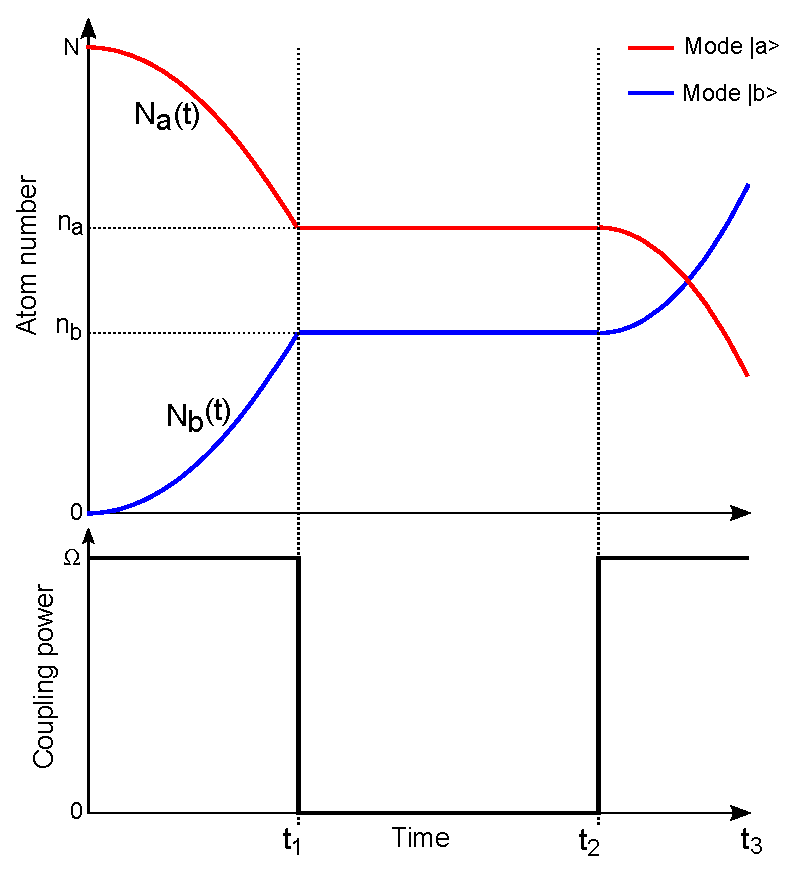
\includegraphics[width=8cm]{figures/pulse_scheme.eps}
    \caption{Mollusc mollusc}
    \label{figPulseScheme}
\end{figure}


\section{Multimode background section}
\begin{itemize}
  \item Motivate why MM analysis is necessary
  \item Brief recap why MM QFT is hard
  \item Say how great phase space methods are, quick overview of how they work, say only wigner works here, can probably crib some explanation and formulae from our fully quantum multimode atom laser paper
  \item Talk about all the checks I've done to make sure Wigner holds over the parameters we've simulated despite the fact that TWA is an uncontrolled approximation
  \item Cite XMDS, and say we're amazing at doing QFT sims, send money
  Derive link between mode shape, nonlinearity U, and the SM equivalent nonlinearity, so we can always compare a given high-dimensional multimode sim against the equivalent ideal analytic single mode case
\end{itemize}

\section{Meanfield multimode problems}
\begin{itemize}
  \item Point out that different densities have phases that evolve at different rates
  \item This leads to poor mode matching when recombining if two states have different nonlinearity*number values 
  \item give a plot of the mode in |a> and |b> at the beginning and end of the hold time to show mismatch
  \item This means constant density is good since mode shape doesn't change
  \item Plot of squeezing for given set of params for gaussian, TF, constant density, show it get steadily better
  \item Say we can use a pi pulse to swap the populations half way through, so if the states have different nonlinearities we still end up with the same mode shapes when we recombine. The fact that this works will be clear from the SM equations for a(t), b(t) when the beam splitter is on
  \item show some plots of squeezing with and without the pi pulse
\end{itemize}

\section{Mean field quantum statistical results}
  \begin{itemize}
  \item Two issues. 1) as we add dimensions results get worse (maybe point out how cool we are for being able to do multimode 3D simulations). 2) As our volume increases results get worse.
  \item To gain insight into this we do a bog analysis
  \item Do a comparision plot between SM analytic model and Bog to show everything agrees
  \item show that the number of mode available degrades squeezing
  \item Plot some bog results v MM sims for increasing box sizes, and increasing dimensions
  \item Can we put some numbers on how bad 3D is compared to 2D, in order to motivate tight trapping?
  \end{itemize}

\section{Mitigating multimode quantum statistical effects}
  \begin{itemize}
  \item One way to approximate constant density is to look at core of BEC, since if we only look at number in the central 1 sigma portion of gaussian it's close to flat; show results compared to single mode equivalent

  \item Another improvement is to put the BEC in a box since then we get constant density, discuss feasibility
  \item 3D still sucks even with box, so point out we can win by freezing out dimensions
  \item Show derivation for what physical situations are needed to freeze out 1, 2 and 3 dimensions. In general we need small number, which makes it hard since we want large number squeezing. Large number requirement leads to implausible geometry in 1D (i.e. a tube with a ridiculous aspect ratio), but going from 3D down to 2D is probably do-able
  \end{itemize}

\section{Conclusion}
\label{sectionConclusion}
\begin{itemize}
  \item Kerr nonlinearities can give arbitrarily good squeezing in BECs with high number
  \item In a straightforward approach we can't get good squeezing with high number due to MM effects
  \item Mode matching issues can be solved with equal scattering lengths or a pi pulse or a box
  \item Another MM effect scales with dimension and physical size
  \item Can solve that problem with tight trapping and box
\end{itemize}

\ack
Acknowledgements in here; funding sources etc

\clearpage

\appendix
\section{Derivation of single mode squeezing formula}
\label{appendixTwoModeDerivation}

\section*{References}
\begin{thebibliography}{10}
\bibitem{gross2010} Gross C, Zibold T, Est{\`{e}}ve J and Oberthaler M K 2010 Nonlinear atom interferometer surpasses classical
precision limit {\it Nature} {\bf 464} 1165--1169
\bibitem{dennis2013} Dennis G R, Hope J J and Johnsson M T 2013 XMDS2: Fast, scalable simulation of coupled stochastic partial
differential equations {\it Comput. Phys. Commun.} {\bf 184} 201--208

\end{thebibliography}

\end{document}

